\section{Laboratory Setup and Methodology}
\label{sec:lab-setup}

% Support compilation either from report/ or from the repository root.
\graphicspath{{../evidence/}{evidence/}}

\subsection{Laboratory Purpose and Scope}

The laboratory was designed to support controlled comparison across the
different stages of the Copy Fail investigation. Its purpose was not merely to
provide a system on which the published proof of concept could be executed.
The environment also needed to preserve a trustworthy reference state, allow a
historically vulnerable state to be reconstructed deliberately, and support
later detection, mitigation, and patch-validation experiments under comparable
conditions.

The design followed four rules. First, all vulnerability-specific activity was
confined to an isolated, privately owned virtual network. Second, the patched
reference system and the vulnerable reproduction target were maintained as
separate virtual machines rather than as successive states of one machine.
Third, reproduction began from a dedicated local account without administrative
privileges, so a later UID~0 result could be compared with a documented
unprivileged starting state. Finally, each experimental phase was treated as a
separate checkpoint and preserved with the applicable combination of command
output, screenshots, configuration artifacts, and integrity manifests.

This design separates the system state used for comparison from the state
being modified during experimentation. It also allows observations from later
phases to be interpreted against documented preconditions instead of relying
on an increasingly mutated virtual machine. The following sections describe
the infrastructure, network isolation, virtual-machine roles, account
separation, experimental sequence, and evidence-handling process used to
maintain that distinction.

\subsection{Infrastructure and Network Isolation}

The laboratory was hosted on a Dell OptiPlex 5070 Micro running Proxmox
VE~9.2.5. The host provided an Intel Core i5-9500T processor and approximately
31~GiB of memory. These specifications establish the scale of the environment,
but the experiment did not depend on specialised hardware. Both Copy Fail test
systems were conventional x86-64 KVM/QEMU virtual machines.

\begin{table}[H]
    \centering
    \caption{Relevant laboratory infrastructure and network roles.}
    \label{tab:lab-infrastructure}
    \small
    \begin{tabularx}{\textwidth}{@{}>{\bfseries}p{0.27\textwidth}Y@{}}
        \toprule
        Component & Configuration and role \\
        \midrule
        Physical host &
        Dell OptiPlex 5070 Micro, Intel Core i5-9500T, approximately 31~GiB RAM \\

        Hypervisor &
        Proxmox VE~9.2.5 using KVM/QEMU virtualization \\

        Laboratory gateway &
        OPNsense virtual firewall separating the management-facing and internal
        laboratory segments \\

        Management bridge &
        \code{vmbr0}, connected to the ordinary management network and to the
        management-facing interface of OPNsense \\

        Internal bridge &
        \code{vmbr1}, providing the isolated Layer-2 segment used by the Copy
        Fail guest systems \\

        Guest attachment &
        A single virtual network interface on \code{vmbr1}; addressing and the
        default gateway were provided within the laboratory subnet \\
        \bottomrule
    \end{tabularx}
\end{table}

The logical network path is shown in \cref{fig:lab-topology}. Private IP
addresses, MAC addresses, and unrelated details of the surrounding home
network are intentionally omitted because they do not affect reproduction of
the experiment.

\begin{figure}[H]
    \centering
    \begin{tikzpicture}[
        infrastructure/.style={
            draw=MoriRule,
            fill=MoriCode,
            text=MoriInk,
            minimum width=6.2cm,
            minimum height=0.9cm,
            align=center,
            font=\displayfont\small
        },
        boundary/.style={
            draw=MoriPurple,
            fill=MoriMist,
            text=MoriInk,
            line width=0.8pt,
            minimum width=6.2cm,
            minimum height=0.95cm,
            align=center,
            font=\displayfont\small\bfseries
        },
        guest/.style={
            draw=MoriRule,
            fill=MoriPaper,
            text=MoriInk,
            minimum width=5.4cm,
            minimum height=1.05cm,
            align=center,
            font=\displayfont\small
        },
        path/.style={
            <->,
            line width=0.75pt,
            draw=MoriMuted
        },
        pathlabel/.style={
            fill=MoriPaper,
            inner sep=2pt,
            text=MoriDeepPurple,
            font=\ttfamily\scriptsize
        }
    ]
        \node[infrastructure] (management) at (0,0)
            {Home / management network};
        \node[boundary] (firewall) at (0,-1.8)
            {OPNsense firewall and laboratory gateway};
        \node[infrastructure] (laboratory) at (0,-3.6)
            {Isolated laboratory LAN};
        \node[guest] (reference) at (-3.15,-5.35)
            {VM 270\\Patched reference system};
        \node[guest] (vulnerable) at (3.15,-5.35)
            {VM 271\\Vulnerable reproduction target};

        \draw[path] (management) -- node[pathlabel] {vmbr0} (firewall);
        \draw[path] (firewall) -- node[pathlabel] {vmbr1} (laboratory);
        \draw[->,line width=0.75pt,draw=MoriMuted]
            (laboratory.south) -- ++(0,-0.45) -| (reference.north);
        \draw[->,line width=0.75pt,draw=MoriMuted]
            (laboratory.south) -- ++(0,-0.45) -| (vulnerable.north);
    \end{tikzpicture}
    \caption{Logical separation between the management network and the Copy
    Fail guest systems.}
    \label{fig:lab-topology}
\end{figure}

Neither Copy Fail guest was attached directly to \code{vmbr0}. Their only
virtual network interface was connected to \code{vmbr1}, so communication
between the laboratory segment and the ordinary management network crossed the
OPNsense policy boundary. This prevented the deliberately vulnerable systems
from sharing the ordinary network's Layer-2 segment while retaining controlled
administrative access when required. The vulnerability itself was exercised
locally inside VM~271; no third-party or internet-facing target formed part of
the test path.

\subsection{Virtual-Machine Roles and State Separation}

The two Copy Fail guests shared a controlled starting configuration. VM~270,
\code{copyfail01}, ran Ubuntu Server 24.04.2 LTS with two virtual CPUs, 4~GiB of
memory, a 32~GiB virtual disk, and one \code{vmbr1} network interface. Once it
had been established as a patched reference, VM~271, \code{copyfail-vuln}, was
created as a full clone. The clone retained the same operating-system lineage
and virtual-hardware profile, but its machine identity and SSH host keys were
regenerated so that the guests no longer shared host identity.

The guest baseline for VM~270 is preserved under
\path{evidence/00-baseline/}. The sanitized hypervisor supplement
\path{evidence-audit/vm270-proxmox-state-public.txt} records its virtual CPU,
memory, disk, \code{vmbr1} attachment, and snapshot ancestry without publishing
the original machine identifiers. The public package does not contain an
equivalent Proxmox configuration transcript for VM~271, so the clone procedure
is reported as laboratory methodology while later phase captures establish the
runtime state actually used for each experiment.

The virtual machines were assigned different roles before reconstruction.
VM~270 was preserved as the known-good comparison system and was not downgraded
or repeatedly reconfigured for exploit testing. VM~271 was the only guest
deliberately modified for vulnerable-kernel reconstruction, reproduction,
detection, mitigation, and validation. \Cref{tab:vm-roles} summarizes this
division.

\begin{table}[H]
    \centering
    \caption{Virtual-machine roles and permitted state changes.}
    \label{tab:vm-roles}
    \small
    \begin{tabularx}{\textwidth}{@{}>{\bfseries\raggedright\arraybackslash}p{0.20\textwidth}p{0.25\textwidth}Y@{}}
        \toprule
        Virtual machine & Experimental role & Permitted state changes \\
        \midrule
        VM 270 \code{copyfail01} &
        Patched reference &
        Preserved as the known-good comparison state; no deliberate
        vulnerable reconstruction \\

        VM 271 \code{copyfail-vuln} &
        Experimental target &
        Vulnerable reconstruction, reproduction, detection, mitigation, and
        validation activities \\
        \bottomrule
    \end{tabularx}
\end{table}

Although the guests were not independent experimental samples, cloning reduced
irrelevant starting differences and state separation protected the reference
from destructive work. Comparisons therefore used a preserved control rather
than an undocumented earlier state of the modified target.

\subsection{Account and Privilege Separation}

Privileged laboratory preparation and unprivileged test execution were assigned
to separate local accounts. The \code{researcher} account, with UID~1000 and
primary GID~1000, provided the administrative context required for kernel
management, package and service configuration, instrumentation, and evidence
collection. Its recorded memberships included the administrative groups
\code{adm}, \code{sudo}, and \code{lxd}. Root authority was used where these
tasks required it, but neither the administrative account nor an existing root
shell formed part of the attacker execution context.

The dedicated \code{labuser} account, with UID~1001 and primary GID~1001,
represented an attacker-controlled but initially unprivileged local foothold.
Its recorded supplementary membership was limited to the ordinary
\code{users} group (GID~100); it was not assigned membership in administrative
groups such as \code{sudo} or \code{lxd}. The threat model therefore assumed
that an attacker had already obtained command execution as this ordinary
account; the preceding compromise was not reproduced. The vulnerable-kernel
reproduction and MORI enforcement trials used this account as their attacker
context. The patched-kernel phase recorded the identity again for each retest
rather than assuming it was unchanged: notably, its Python retest used the
\code{researcher} account. That run can show that no automatic UID~0 transition
was observed in its recorded context, but it is not an identity-matched repeat
of the vulnerable \code{labuser} execution. \Cref{tab:account-roles} summarizes
the resulting separation of duties.

\begin{table}[H]
    \centering
    \caption{Account roles and privilege contexts used in the laboratory.}
    \label{tab:account-roles}
    \small
    \begin{tabularx}{\textwidth}{@{}>{\bfseries\raggedright\arraybackslash}p{0.20\textwidth}p{0.28\textwidth}Y@{}}
        \toprule
        Account & Starting context & Laboratory role \\
        \midrule
        \code{researcher} (UID 1000) &
        Administrative; member of \code{adm}, \code{sudo}, and \code{lxd} &
        Environment preparation, instrumentation, and privileged evidence
        collection \\

        \code{labuser} (UID 1001; GID 1001) &
        Unprivileged local user; supplementary membership limited to
        \code{users} (GID 100) &
        Primary attacker context for vulnerable-kernel reproduction and
        compensating-control tests \\
        \bottomrule
    \end{tabularx}
\end{table}

The \code{researcher} state is recorded under
\path{evidence/00-baseline/} in \path{command-output/id.txt}. The
\code{labuser} state is recorded under \path{evidence/02-reproduction/} in
\path{artifacts/01-pre-exploit-state.txt}. Later retests preserve their own
identity captures where the execution context differs.

\begin{figure}[H]
    \centering
    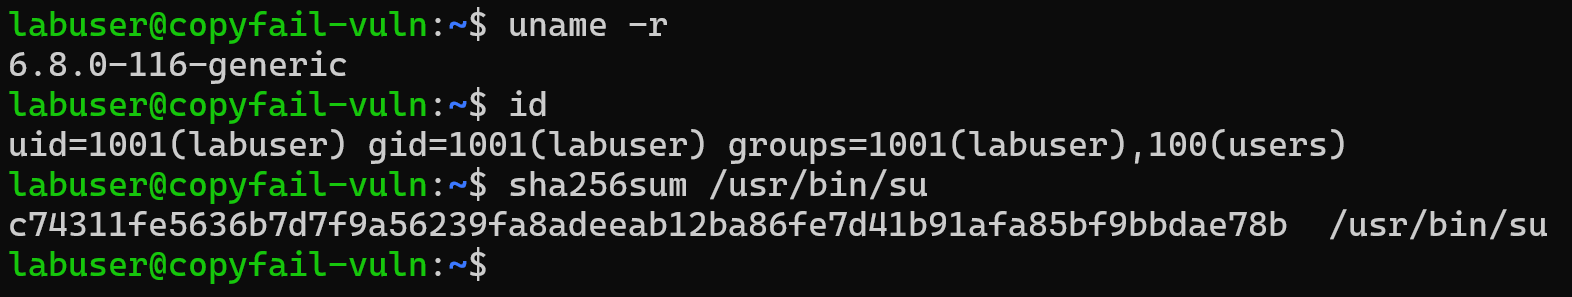
\includegraphics[
        width=\textwidth,
        height=0.36\textheight,
        keepaspectratio
    ]{02-reproduction/screenshots/01-pre-exploit-state.png}
    \caption{Recorded vulnerable-kernel starting state: kernel
    \code{6.8.0-116-generic}, \code{labuser} as UID~1001, its non-administrative
    group membership, and the baseline digest of \code{/usr/bin/su}.}
    \label{fig:labuser-pre-exploit-state}
\end{figure}

The screenshot in \cref{fig:labuser-pre-exploit-state} is the visual capture
paired with the machine-readable pre-exploit artifact. Together they establish
the starting privilege boundary used for the vulnerable-kernel reproduction.

Before each relevant trial, the active identity and privilege state were
recorded from the test account. Keeping preparation and execution contexts
separate prevents an inherited administrative session, a \code{sudo}-launched
process, or a pre-existing root shell from being mistaken for successful local
privilege escalation. Any later change in effective privilege could therefore
be evaluated against the identity recorded for that trial rather than being
confused with laboratory setup.

\subsection{Threat Model and Security Objectives}

The threat model begins after initial access has already occurred. The attacker
is assumed to control the local \code{labuser} account and therefore starts with
command execution as UID~1001 rather than with administrative authority. From
this foothold, the attacker may execute arbitrary local programs, invoke kernel
interfaces available to an ordinary user, and interact with readable privileged
executables. The attacker may also choose the proof-of-concept implementation,
create processes or threads, arrange relevant system calls, and introduce
delays under their control. The preceding compromise of \code{labuser} is an
assumed precondition and is not itself reproduced.

At the start of an attempt, the attacker does not possess UID~0, membership in
\code{sudo} or \code{lxd}, administrative credentials, or ordinary write access
to the targeted SUID executable. The relevant trust boundary is therefore the
transition from the unprivileged UID~1001 context to root authority. Copy Fail
threatens that boundary by combining the accessible AF\_ALG AEAD and
\code{splice()} paths with modification of file-backed page-cache contents
belonging to a readable privileged executable. The protected assets are both
the integrity of privileged executable code and the authority obtained when
that code is executed with UID~0.

The experiment evaluates the objectives in \cref{tab:security-objectives}.
These criteria distinguish observation from enforcement and separate a
compensating control from correction of the underlying kernel flaw.

\begin{table}[H]
    \centering
    \caption{Security objectives derived from the experimental threat model.}
    \label{tab:security-objectives}
    \small
    \begin{tabularx}{\textwidth}{@{}>{\bfseries\raggedright\arraybackslash}p{0.22\textwidth}Y@{}}
        \toprule
        Objective & Required property \\
        \midrule
        Privilege-boundary protection &
        Prevent an unauthorised transition from the documented UID~1001
        starting context to UID~0. \\

        Executable integrity &
        Preserve the contents and security-relevant state of the targeted
        privileged executable during a prevented attempt. \\

        Behavioural detection &
        Identify the exploitation behaviour without depending on a particular
        proof-of-concept filename, programming language, or executable hash. \\

        Selective correlation &
        Associate the relevant operations within the attacker-controlled
        execution context while avoiding attribution across unrelated
        processes and remaining robust against attacker-controlled timing. \\

        Compatibility &
        Preserve the specific benign interface operations selected for control
        testing and state clearly which wider functionality was not exercised. \\

        Patch independence &
        Verify that a corrected kernel prevents the tested escalation path
        without relying on the custom compensating control. \\
        \bottomrule
    \end{tabularx}
\end{table}

Observation alone does not satisfy the prevention objective. A mechanism is
treated as preventive only if it interrupts the attempted privilege escalation
and the protected target retains its integrity. Likewise, the custom
compensating control is expected to act on the correlated exploitation path
rather than on one known proof-of-concept artifact. Compatibility is evaluated
separately so that removing the vulnerable interface and selectively
restricting its dangerous use are not treated as equivalent defensive
properties. In this report, compatibility means only the operations exercised
by the documented controls; it is not a claim about every \code{AF\_ALG} or AEAD
workload.

The model excludes the means by which \code{labuser} was initially compromised,
remote exploitation, persistence, credential collection, reverse shells,
lateral movement, container escape, unrelated privilege-escalation techniques,
and post-root activity beyond the minimal evidence needed to establish the
privilege state. These exclusions keep the analysis focused on whether control
of an ordinary local account can be escalated through Copy Fail, and whether the
evaluated defences prevent that transition under the stated conditions.

\subsection{Experimental Sequence and State Transitions}

The investigation was organised as a sequence of controlled system states
rather than as one continuous session on an increasingly modified machine.
VM~270 remained the patched reference, while VM~271 was moved deliberately
through vulnerable reconstruction, reproduction, observation, mitigation, and
final patch-validation states. This separation provided a stable comparison
system and made the state-changing work on VM~271 explicit.

Each phase followed the same control cycle. A relevant snapshot or documented
checkpoint was first established or restored. The running kernel, required
interfaces, active account, defensive-control state, and protected target were
then checked as applicable to that phase. Evidence was collected around the
phase-specific activity, with pre-test and post-test captures used where they
were available and relevant. The resulting artifacts were preserved before
another kernel, configuration, or control change was introduced.
\Cref{tab:experimental-sequence} maps this procedure to the six public evidence
sets used by the report.

\begin{table}[H]
    \centering
    \caption{Controlled experimental sequence and state transitions.}
    \label{tab:experimental-sequence}
    \small
    \begin{tabularx}{\textwidth}{@{}>{\bfseries\raggedright\arraybackslash}p{0.16\textwidth}>{\raggedright\arraybackslash}p{0.29\textwidth}Y@{}}
        \toprule
        Evidence set & Established state & Methodological purpose \\
        \midrule
        Phase 00 &
        VM~270 preserved as the patched reference &
        Record a known-good comparison state that was not subjected to
        vulnerable reconstruction or exploit development. \\

        Phase 01 &
        VM~270 checked against the Copy Fail prerequisites and vendor state &
        Record which relevant interfaces, modules, package rules, and fixed
        kernel state were present before building the vulnerable target. \\

        Phase 02 &
        VM~271 booted into the selected historical kernel with the required
        Copy Fail interfaces available and no specific enforcement active &
        Verify the vulnerable preconditions, execute from the documented
        UID~1001 context, and record the privilege and target states. \\

        Phase 03 &
        Reproducible vulnerable state with monitoring introduced separately
        from enforcement &
        Identify observable behaviour, evaluate integrity-based monitoring,
        and compare behavioural evidence with artifact-specific detection. \\

        Phase 04 &
        Vulnerable kernel with broad restriction followed by successive MORI
        observation, correlation, shadow, and enforcement candidates &
        Compare interface removal with selective control, exercise positive and
        negative regression cases, and freeze the final vulnerable-kernel
        candidate. \\

        Phase 05 &
        VM~271 updated to the corrected kernel with MORI isolated from the
        active enforcement path &
        Record the identity used for each retest, exercise the tested interface
        operations, and repeat both proof-of-concept paths independently of the
        custom control. \\
        \bottomrule
    \end{tabularx}
\end{table}

The phase numbers correspond directly to the directories under
\path{evidence/}. Phase~04 contains several internal MORI checkpoints because
control development required more than one state transition, but those
checkpoints are engineering iterations rather than independent experimental
samples.

The order of these transitions was significant. Unmitigated reproduction was
completed before preventive mechanisms were introduced, ensuring that later
denials could be compared with a demonstrated vulnerable path. Monitoring was
introduced before selective enforcement so that candidate observables and
correlation rules could be examined without initially changing the tested
operation. Broad interface restriction showed the effect on the interface
operations selected for testing, whereas the later MORI stages progressively
narrowed the controlled behaviour through observation, correlation, shadow
evaluation, and active enforcement.

Regression testing was treated as part of control development rather than as a
single final exploit run. Trials varied the proof-of-concept implementation,
process or thread context, operation ordering, attacker-controlled delay, and
privileged target where the phase required it. Negative controls were retained
to distinguish the correlated Copy Fail path from isolated or unrelated uses of
the same system interfaces. A candidate was not treated as the current MORI
implementation until these phase-specific checks had been performed against a
documented build and system state.

Vendor remediation was applied only after the vulnerable-kernel experiments
and their checkpoints had been preserved. Isolation of MORI from the active
enforcement path was a required condition of the patched-kernel retest. The
evidence for its exact timing is not perfect: a screenshot shows the isolated
state in the retest sequence, while the timestamped machine-readable capture
was collected later. The patched result is therefore interpreted from the
combined state and execution records rather than from that timestamp alone.
The affected interface was checked separately at the \code{socket()},
\code{bind()}, and \code{accept()} stages. This confirms availability of those
tested operations, not a complete encrypt/decrypt round trip.

The phases form a dependent engineering and validation sequence rather than a
set of independent statistical samples. Their evidential value therefore rests
on the documented preconditions and adjacent pre-test and post-test captures.
Observations made after a state transition were not retroactively used to
characterise an earlier phase; where a later test exposed a new condition, that
condition was added as a prospective regression case and recorded in the state
in which it was actually exercised.

\subsection{Evidence Collection, Integrity, and Publication Workflow}

Evidence was collected alongside each experimental phase and kept separate
from the analytical report. Phase directories normally combined
machine-readable artifacts, screenshots, explanatory documentation, and an
integrity manifest. This structure allowed later claims to be traced to their
preconditions, execution, and post-test records without treating the report
narrative as primary evidence.

The evidence classes in \cref{tab:evidence-classes} served complementary
purposes; no single class was considered sufficient for every claim.

\begin{table}[H]
    \centering
    \caption{Evidence classes and their methodological roles.}
    \label{tab:evidence-classes}
    \small
    \begin{tabularx}{\textwidth}{@{}>{\bfseries\raggedright\arraybackslash}p{0.21\textwidth}>{\raggedright\arraybackslash}p{0.32\textwidth}Y@{}}
        \toprule
        Evidence class & Primary function & Inherent limitation \\
        \midrule
        Command output and logs &
        Preserve searchable kernel, identity, service, event, permission, and
        target state. &
        Only the requested commands are represented; collection can fail or
        omit context. \\

        Screenshots &
        Preserve visible terminal context, ordering, concurrent telemetry, and
        interactive outcomes. &
        Captures are selective and may omit timestamps or complete output. \\

        Configuration and source &
        Record relevant detectors, mitigations, services, policies, and test
        material. &
        Source does not establish which build was loaded or exercised. \\

        Build and provenance records &
        Associate source, generated objects, binaries, compiler context,
        revisions, and digests. &
        Provenance identifies a candidate but does not prove its runtime
        behaviour. \\

        Snapshots and checkpoints &
        Preserve recoverable system states and historical MORI implementations. &
        A checkpoint establishes recoverability, not an experimental claim
        without adjacent captures. \\
        \bottomrule
    \end{tabularx}
\end{table}

For state-changing trials, evidence was collected around the test rather than
only afterwards. Applicable pre-test captures identified the kernel, account,
interface or module state, defensive-control state, and privileged target.
Execution output and telemetry were followed by the resulting privilege and
target state. Where chronology was material, timestamps were included inside
the capture when practicable; file-system and archive modification times were
supporting metadata rather than the sole proof of event order.

Evidence numbering and phase maps preserved the recorded sequence. Missing or
removed items were not hidden by renumbering later objects. A supplemental
capture could clarify a retained state or artifact, but could not retroactively
establish an uncaptured precondition. It therefore required explicit labelling
rather than being presented as part of the original sequence. Filenames were
treated as navigation aids, not as proof of system state. If a filename and its
captured contents disagreed, the commands and output inside the capture governed
the interpretation.

Implementation provenance remained separate from runtime results. MORI
checkpoints preserved successive source, generated BPF objects, skeletons, and
userspace builds, while the validated candidate was placed under the distinct
\code{current/} path. Digests and provenance records associated the frozen
source and build artifacts with the candidate used for final regression.
Proof-of-concept provenance used available repository revisions, source and
binary hashes, compiler information, and execution captures without requiring
redistribution of the exploit implementation.

Integrity protection followed a two-stage workflow. Raw evidence was hashed
before the private original was preserved. Publication work then occurred on a
separate copy. After redaction, omission, renaming, or other sanitization, the
public package received its own SHA-256 manifest and was verified again after
assembly or transfer. Private and public digests were not interchangeable
because legitimate publication transformations change the affected bytes.

\begin{figure}[H]
    \centering
    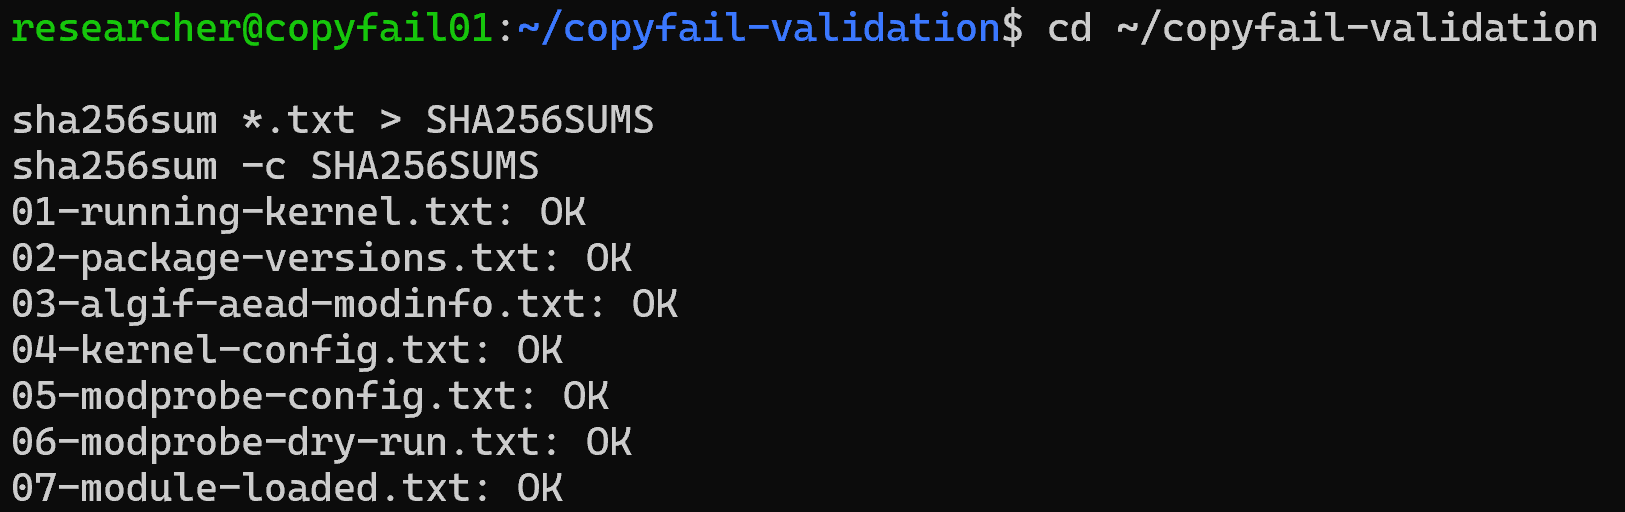
\includegraphics[
        width=\textwidth,
        height=0.46\textheight,
        keepaspectratio
    ]{01-vulnerability-validation/screenshots/01-validation-integrity-check.png}
    \caption{Phase~01 command-output files verified against their recorded
    SHA-256 list. This capture illustrates the integrity check used around the
    experimental evidence packages.}
    \label{fig:phase01-evidence-integrity-check}
\end{figure}

Manifest scope was defined per package. The manifest was excluded from its own
coverage, while editable documentation could be included or explicitly
excluded according to the phase. A file beside
\code{PUBLIC-SHA256SUMS.txt} was therefore not automatically covered;
verification used the manifest's enumerated paths. A filename or object change
after manifest generation invalidated that entry until the manifest was updated.
Verification results were therefore recorded entry by entry rather than
summarized from the mere presence of a manifest.

SHA-256 verification was a change-detection mechanism, not proof that a capture
was complete or correctly interpreted. A matching digest shows that the checked
bytes correspond to the listed version. It does not establish when a command
ran, whether it captured the intended property, whether a screenshot omitted
context, or whether documentation describes the artifact accurately. Content
review and cryptographic verification were separate publication gates.

The public copy was reviewed for credentials, tokens, internal network details,
machine identifiers, and unrelated environmental information. Exploit source
or other unnecessary material could be withheld while retaining hashes,
provenance, system state, and execution outcomes. Omissions were documented,
numbering gaps were preserved where useful, and publication edits did not
overwrite the unsanitized original.

Incomplete captures were retained and described according to their contents. A
failed text capture stayed failed even when a contemporaneous screenshot
preserved the missing result. The screenshot could supplement the record, but
it did not rewrite the status of the original artifact. Screenshot-only runs
also remained screenshot-only; no replacement transcript was created after the
fact.

This workflow supports internal traceability and change detection, but is not a
formal forensic acquisition with an independent trusted timestamp,
hardware-backed attestation, or external witness. Later claims are therefore
limited to the properties preserved by the cited artifacts and to the
controlled laboratory states in which they were collected.